\documentclass[aspectratio=1610]{beamer}
\usetheme{Madrid}


\usepackage{amsmath}
\usepackage{amssymb}
\usepackage{listings}
\usepackage{booktabs}
\usepackage{multirow}
\usepackage{multirow}
\usepackage{lmodern}
\usepackage{xcolor}
\usepackage{float}
\lstset{
  language=Python,  %代码语言使用的是matlab
  % frame=shadowbox, %把代码用带有阴影的框圈起来
  rulesepcolor=\color{red!20!green!20!blue!20},%代码块边框为淡青色
  keywordstyle=\color{blue!90}\bfseries, %代码关键字的颜色为蓝色,粗体
  commentstyle=\color{red!10!green!70}\textit,    % 设置代码注释的颜色
  basicstyle=\footnotesize,
  showstringspaces=true,%不显示代码字符串中间的空格标记
  % numbers=left, % 显示行号
  % numberstyle=8pt,    % 行号字体
  % numberstyle=\color{green},
  stringstyle=\rmfamily\slshape\color[RGB]{128,0,0}, % 代码字符串的特殊格式
  breaklines=true, %对过长的代码自动换行
  extendedchars=false,  %解决代码跨页时,章节标题,页眉等汉字不显示的问题
  escapeinside=``,%代码中出现中文必须加上,否则报错
  texcl=true}

\lstset{breaklines}%自动将长的代码行换行排版

\lstset{extendedchars=false}%解决代码跨页时,章节标题,页眉等汉字不显示的问题

\usepackage{textcomp}
% \usepackage[margin=1in]{geometry}
\usepackage{pythonhighlight}
% \usepackage{minted}
\usepackage[backend=bibtex]{biblatex}
%\usepackage[style=authortitle,backend=biber]{biblatex}
\addbibresource{ResearchRabbit_Export_2022_10_20.bib}

\usepackage{algorithm}
\usepackage{algorithmic}
\renewcommand{\algorithmicrequire}{\textbf{Input:}}
\renewcommand{\algorithmicensure}{\textbf{Output:}}


\title[logic synthesis libraries]{The EPFL Logic Synthesis Libraries}
\author[Gcc]{Dingchao Gao}
\institute[ISCAS]{Institute of Software Chinese Academy of Sciences}

\begin{document}

\begin{frame}[plain]
  \titlepage
  %  Title page
\end{frame}

\section{induction}
\begin{frame}
  SIS, 
\end{frame}

\section{tweedledum}
\begin{frame}{induction}  
  ABC 
\end{frame}
\begin{frame}{compilation flow}
  \begin{figure}[htbq]
    \centering
    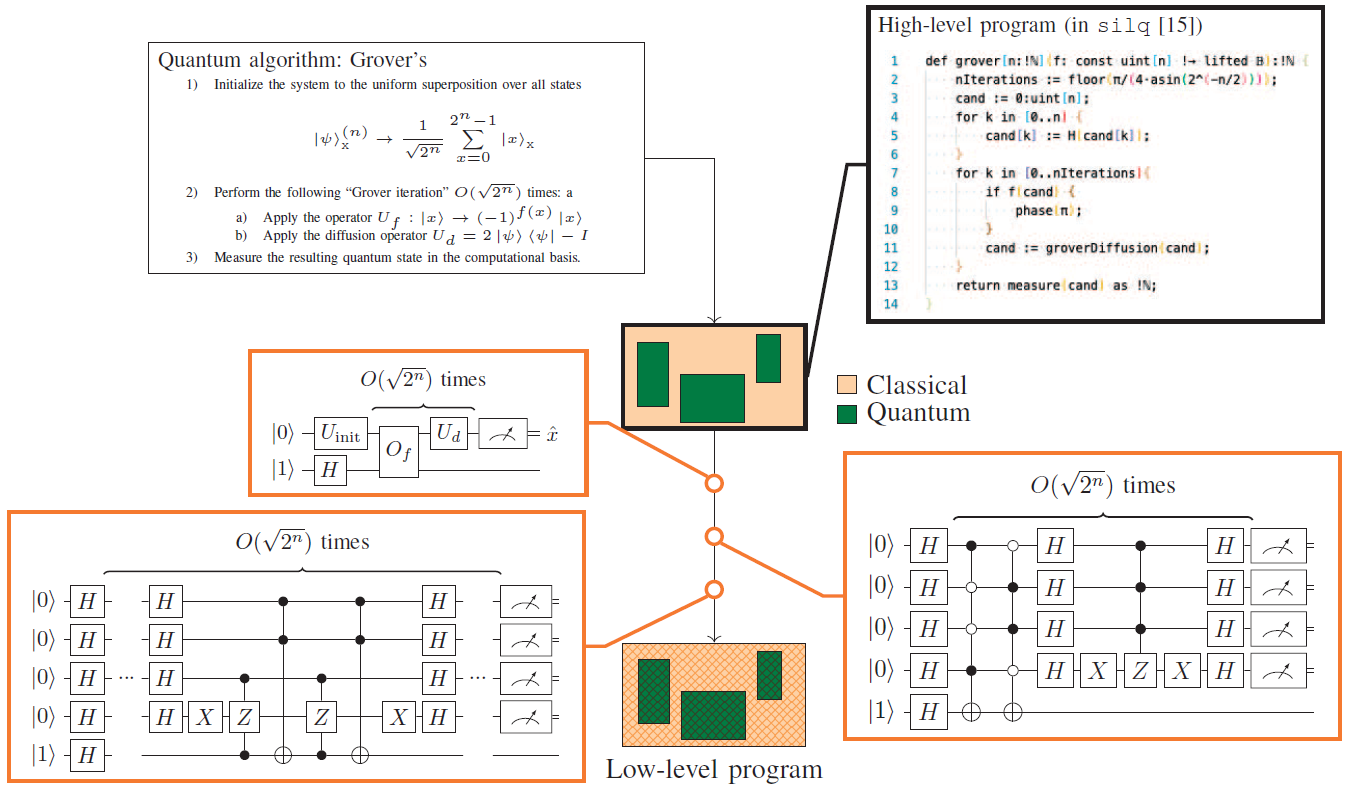
\includegraphics[width=0.8\textwidth]{figure/work_flow.png}
    \caption{compilation flow overview} 
    \label{fig-compilation}
  \end{figure}
\end{frame}
\begin{frame}{flexibility}
  \begin{figure}[htbq]
    \centering
    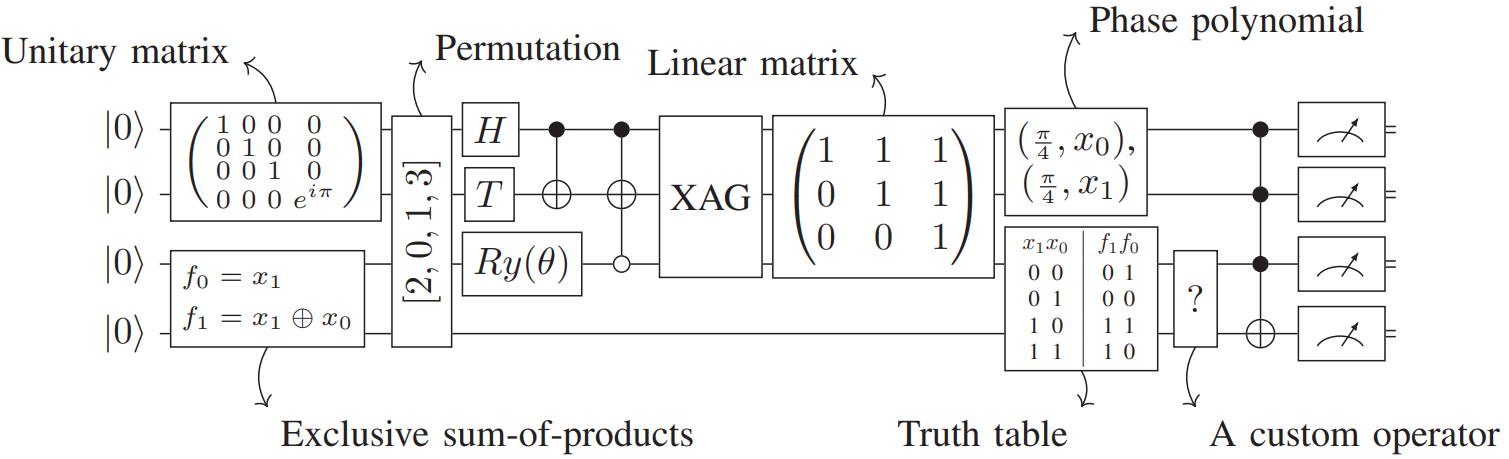
\includegraphics[width=0.9\textwidth]{figure/flex.png}
    \caption{tweedledum's IR flexibility} 
    \label{fig-flex}
  \end{figure}
\end{frame}
\begin{frame}{synthesis}
  \begin{itemize}
    \item 
  \end{itemize}  
\end{frame}
\begin{frame}{synthesis}
  \begin{figure}[htbq]
    \centering
    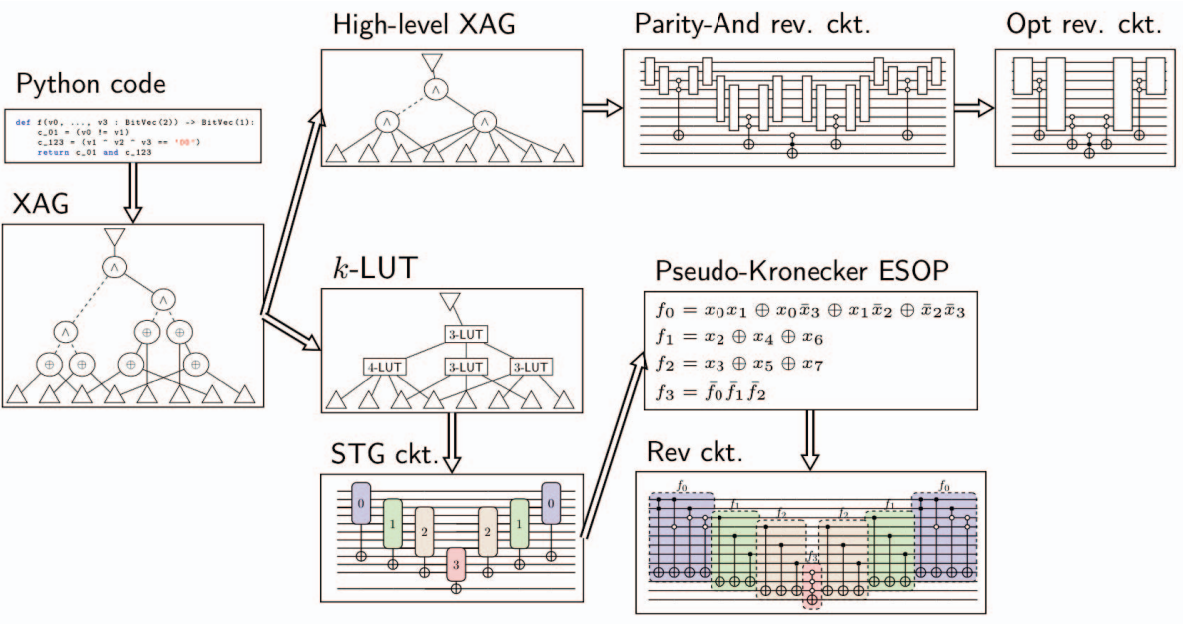
\includegraphics[width=0.7\textwidth]{figure/boolean.png}
    \caption{overview of possible Boolean function synthesis flows} 
    \label{fig-boolean}
  \end{figure}
\end{frame}
\begin{frame}{compilation passes}
  \begin{itemize}
    \item 
  \end{itemize}
\end{frame}

\section{Protocol Example}
\subsection{a protocol of leader in network}
\subsection{loop}

\begin{frame}{disscussio}
  \begin{itemize}
    \item lack of quantum computing features
    \item comparing with isq etc
    \item the abstract level of quantum computer? 
  \end{itemize}
\end{frame}

\begin{frame}[noframenumbering,allowframebreaks,t]
	\frametitle{references}
	\printbibliography
\end{frame}

\begin{frame}
\centering
\Huge{END\\Thank you}
\end{frame}
\end{document}